\documentclass{beamer}
\usepackage{amsmath}
\usepackage{amssymb}
\usepackage{microtype}
\usepackage{siunitx}
\usepackage[style=english=british]{csquotes}
\usefonttheme[onlymath]{serif}
\sisetup{exponent-product = \cdot}

\author{S. Bodapati \and D. Jain \and S. Malhan \and A. Shokeen}
\date{2026-01-20}
\title{Redshift Reduction Telescope: Prototype presentation}

\begin{document}

\maketitle

\begin{frame}
    \frametitle{Why have the researchers built this?}
    The researchers have built this to aid in the reduction of cosmological redshift; it is described above, and is a serious problem in astronomical imaging. According to Jain, \enquote{enhance our \emph{interpretation} of} redshift, removing it via software to allow for a nicer view of the universe. The researchers wanted to help astrophotographers and hobbyists who like taking pictures of the universe. Our prototype shall fix this using software reconstruction in the concise language Python, with the help of libraries such as OpenCV. This is a great tool for astrophotographers and hobbyists.
\end{frame}

\begin{frame}
    \frametitle{What is redshift?}
    The researchers (us) are attempting to solve the problem of cosmological redshift. Redshift is mathematically defined as \pause\[
    z = \frac{\lambda_{\text{observed}}}{\lambda_{\text{emitted}}} - 1,
    \]\pause and it is the phenomenon where light emitted from distant astronomical electromagnetic radiators is stretched out by the universe's expansion. This affects astronomical imaging, which is a complication in accurately imaging the observable universe. \pause For example, the redshift of a galaxy 2 \unit{\yotta\metre} away emitting a wavelength of 400 \unit{\nano\metre} can be calculated through:\pause
    \begin{align*}
        v &= H_0 \cdot d\\
        v &\approx (\num{2.23e-18}) \cdot (\num{2e24}) \unit{\metre\per\second}\\
        v &\approx \num{4.46e6} \unit{\metre\per\second}
    \end{align*}
\end{frame}

\begin{frame}
    \frametitle{What is redshift? --- continued}
    The velocity of the galaxy has been obtained. Now, using the relativistic redshift formula:
    \begin{align*}
        z &= (1 + \frac{v}{c})\frac{1}{\sqrt{1 - \frac{v^2}{c^2}}}\\
        % oh dear my calculator :(
        z &\approx (1 + \frac{\num{4.46e6}}{\num{3e8}})\frac{1}{\sqrt{1 - \frac{(\num{4.46e6})^2}{(\num{3e8})^2}}}\\
        z &\approx 1.015
    \end{align*}
    Applying this to the original wavelength:
    \begin{align*}
        \lambda_{obs} &= z\lambda_{emit}\\
        \lambda_{obs} &\approx (\num{4e-7})(\num{1.015})\\
        \lambda_{obs} &\approx \num{4.06e-7} \unit{\metre}
    \end{align*}
\end{frame}
\begin{frame}
    \frametitle{What is redshift? --- continued\textsuperscript{2}}
    Redshift, put simply, is but a distortion; a stretching of light, due to the expansion of the universe. The below diagram explains redshift concisely:
    \begin{figure}
        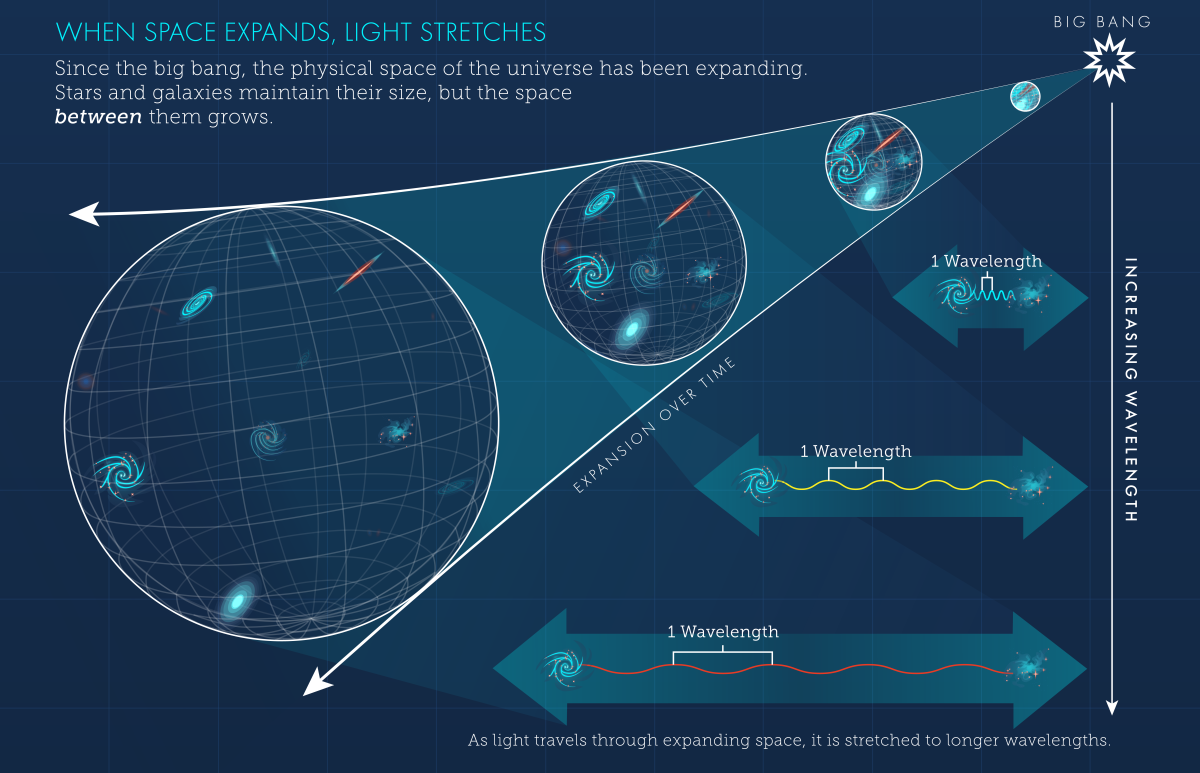
\includegraphics[width=7.5cm]{images/redshift-diagram.png}
        \caption{Redshift. Source: NASA, ESA, and Leah Hustak from STScl.}
    \end{figure} 
\end{frame}
\begin{frame}
    \frametitle{Mechanism and operation: building}
    The researchers shall use a standard refracting telescope; they shall buy a pre-built telescope, due to the relatively lower cost. T
\end{frame}

\end{document}